\documentclass[conference]{IEEEtran}
\usepackage{cite}
\usepackage{amsmath,amssymb}
\usepackage{graphicx}
\usepackage{booktabs}
\usepackage{url}
\usepackage{textcomp}
\usepackage[T1]{fontenc}
\hyphenation{GNSS}
\newcommand{\nFonefourBgatediff}{-0.105}
\newcommand{\nFonefourBgatehi}{-0.025}
\newcommand{\nFonefourBgatelo}{-0.194}
\newcommand{\nFonefourBgatep}{0.0153}
\newcommand{\nFonefourBtwodiff}{0.087}
\newcommand{\nFonefourBtwohi}{0.126}
\newcommand{\nFonefourBtwolo}{0.032}
\newcommand{\nFonefourBtwop}{0.0034}
\newcommand{\nFonefourBzerodiff}{-1.680}
\newcommand{\nFonefourBzerohi}{-0.577}
\newcommand{\nFonefourBzerolo}{-2.675}
\newcommand{\nFonefourBzerop}{0.0001}
\newcommand{\nFoneoneBgatediff}{-0.060}
\newcommand{\nFoneoneBgatehi}{-0.032}
\newcommand{\nFoneoneBgatelo}{-0.100}
\newcommand{\nFoneoneBgatep}{0.0000}
\newcommand{\nFoneoneBtwodiff}{0.029}
\newcommand{\nFoneoneBtwohi}{0.055}
\newcommand{\nFoneoneBtwolo}{0.015}
\newcommand{\nFoneoneBtwop}{0.0000}
\newcommand{\nFoneoneBzerodiff}{-0.521}
\newcommand{\nFoneoneBzerohi}{-0.232}
\newcommand{\nFoneoneBzerolo}{-0.768}
\newcommand{\nFoneoneBzerop}{0.0002}
\newcommand{\nFonethreeBgatediff}{-0.110}
\newcommand{\nFonethreeBgatehi}{-0.063}
\newcommand{\nFonethreeBgatelo}{-0.183}
\newcommand{\nFonethreeBgatep}{0.0000}
\newcommand{\nFonethreeBtwodiff}{0.042}
\newcommand{\nFonethreeBtwohi}{0.085}
\newcommand{\nFonethreeBtwolo}{0.021}
\newcommand{\nFonethreeBtwop}{0.0000}
\newcommand{\nFonethreeBzerodiff}{-0.981}
\newcommand{\nFonethreeBzerohi}{-0.199}
\newcommand{\nFonethreeBzerolo}{-1.661}
\newcommand{\nFonethreeBzerop}{0.0002}
\newcommand{\nFonetwoBgatediff}{-0.082}
\newcommand{\nFonetwoBgatehi}{-0.063}
\newcommand{\nFonetwoBgatelo}{-0.162}
\newcommand{\nFonetwoBgatep}{0.0000}
\newcommand{\nFonetwoBtwodiff}{0.034}
\newcommand{\nFonetwoBtwohi}{0.058}
\newcommand{\nFonetwoBtwolo}{0.013}
\newcommand{\nFonetwoBtwop}{0.0000}
\newcommand{\nFonetwoBzerodiff}{-0.250}
\newcommand{\nFonetwoBzerohi}{0.049}
\newcommand{\nFonetwoBzerolo}{-0.951}
\newcommand{\nFonetwoBzerop}{0.0184}
\newcommand{\nFonezeroBgatediff}{-0.048}
\newcommand{\nFonezeroBgatehi}{-0.016}
\newcommand{\nFonezeroBgatelo}{-0.066}
\newcommand{\nFonezeroBgatep}{0.0009}
\newcommand{\nFonezeroBtwodiff}{0.008}
\newcommand{\nFonezeroBtwohi}{0.018}
\newcommand{\nFonezeroBtwolo}{-0.002}
\newcommand{\nFonezeroBtwop}{0.0627}
\newcommand{\nFonezeroBzerodiff}{-0.093}
\newcommand{\nFonezeroBzerohi}{-0.002}
\newcommand{\nFonezeroBzerolo}{-0.152}
\newcommand{\nFonezeroBzerop}{0.0627}
\newcommand{\nFthreefourcoverA}{0.226}
\newcommand{\nFthreefourcoverB}{0.093}
\newcommand{\nFthreefourcoverdiff}{0.068}
\newcommand{\nFthreefourcoverp}{0.0193}
\newcommand{\nFthreefourdriftA}{2.613}
\newcommand{\nFthreefourdriftB}{3.257}
\newcommand{\nFthreefourdriftdiff}{0.064}
\newcommand{\nFthreefourdriftp}{1.0000}
\newcommand{\nFthreeonecoverA}{0.157}
\newcommand{\nFthreeonecoverB}{0.077}
\newcommand{\nFthreeonecoverdiff}{0.018}
\newcommand{\nFthreeonecoverp}{0.0119}
\newcommand{\nFthreeonedriftA}{0.988}
\newcommand{\nFthreeonedriftB}{1.035}
\newcommand{\nFthreeonedriftdiff}{-0.001}
\newcommand{\nFthreeonedriftp}{1.0000}
\newcommand{\nFthreethreecoverA}{0.067}
\newcommand{\nFthreethreecoverB}{0.022}
\newcommand{\nFthreethreecoverdiff}{0.009}
\newcommand{\nFthreethreecoverp}{0.0186}
\newcommand{\nFthreethreedriftA}{1.762}
\newcommand{\nFthreethreedriftB}{1.733}
\newcommand{\nFthreethreedriftdiff}{-0.116}
\newcommand{\nFthreethreedriftp}{1.0000}
\newcommand{\nFthreetwocoverA}{0.118}
\newcommand{\nFthreetwocoverB}{0.060}
\newcommand{\nFthreetwocoverdiff}{0.048}
\newcommand{\nFthreetwocoverp}{0.0012}
\newcommand{\nFthreetwodriftA}{1.289}
\newcommand{\nFthreetwodriftB}{1.372}
\newcommand{\nFthreetwodriftdiff}{0.019}
\newcommand{\nFthreetwodriftp}{1.0000}
\newcommand{\nFthreezerocoverA}{0.065}
\newcommand{\nFthreezerocoverB}{0.046}
\newcommand{\nFthreezerocoverdiff}{0.007}
\newcommand{\nFthreezerocoverp}{0.0904}
\newcommand{\nFthreezerodriftA}{0.897}
\newcommand{\nFthreezerodriftB}{0.878}
\newcommand{\nFthreezerodriftdiff}{0.023}
\newcommand{\nFthreezerodriftp}{1.0000}
\newcommand{\nFtwofourBgatediff}{-0.37}
\newcommand{\nFtwofourBgatehi}{-0.14}
\newcommand{\nFtwofourBgatelo}{-0.60}
\newcommand{\nFtwofourBgatep}{0.0004}
\newcommand{\nFtwofourBtwodiff}{0.38}
\newcommand{\nFtwofourBtwohi}{0.50}
\newcommand{\nFtwofourBtwolo}{0.20}
\newcommand{\nFtwofourBtwop}{0.0000}
\newcommand{\nFtwofourBzerodiff}{-7.48}
\newcommand{\nFtwofourBzerohi}{-6.31}
\newcommand{\nFtwofourBzerolo}{-10.58}
\newcommand{\nFtwofourBzerop}{0.0000}
\newcommand{\nFtwooneBgatediff}{-0.17}
\newcommand{\nFtwooneBgatehi}{-0.13}
\newcommand{\nFtwooneBgatelo}{-0.29}
\newcommand{\nFtwooneBgatep}{0.0000}
\newcommand{\nFtwooneBtwodiff}{0.04}
\newcommand{\nFtwooneBtwohi}{0.10}
\newcommand{\nFtwooneBtwolo}{0.02}
\newcommand{\nFtwooneBtwop}{0.0002}
\newcommand{\nFtwooneBzerodiff}{-2.00}
\newcommand{\nFtwooneBzerohi}{-1.63}
\newcommand{\nFtwooneBzerolo}{-3.25}
\newcommand{\nFtwooneBzerop}{0.0000}
\newcommand{\nFtwothreeBgatediff}{-0.33}
\newcommand{\nFtwothreeBgatehi}{-0.26}
\newcommand{\nFtwothreeBgatelo}{-0.59}
\newcommand{\nFtwothreeBgatep}{0.0000}
\newcommand{\nFtwothreeBtwodiff}{0.15}
\newcommand{\nFtwothreeBtwohi}{0.22}
\newcommand{\nFtwothreeBtwolo}{0.08}
\newcommand{\nFtwothreeBtwop}{0.0000}
\newcommand{\nFtwothreeBzerodiff}{-6.00}
\newcommand{\nFtwothreeBzerohi}{-3.30}
\newcommand{\nFtwothreeBzerolo}{-7.67}
\newcommand{\nFtwothreeBzerop}{0.0000}
\newcommand{\nFtwotwoBgatediff}{-0.23}
\newcommand{\nFtwotwoBgatehi}{-0.17}
\newcommand{\nFtwotwoBgatelo}{-0.41}
\newcommand{\nFtwotwoBgatep}{0.0000}
\newcommand{\nFtwotwoBtwodiff}{0.07}
\newcommand{\nFtwotwoBtwohi}{0.17}
\newcommand{\nFtwotwoBtwolo}{0.05}
\newcommand{\nFtwotwoBtwop}{0.0000}
\newcommand{\nFtwotwoBzerodiff}{-2.79}
\newcommand{\nFtwotwoBzerohi}{-1.77}
\newcommand{\nFtwotwoBzerolo}{-3.78}
\newcommand{\nFtwotwoBzerop}{0.0000}
\newcommand{\nFtwozeroBgatediff}{-0.14}
\newcommand{\nFtwozeroBgatehi}{-0.12}
\newcommand{\nFtwozeroBgatelo}{-0.17}
\newcommand{\nFtwozeroBgatep}{0.0000}
\newcommand{\nFtwozeroBtwodiff}{0.04}
\newcommand{\nFtwozeroBtwohi}{0.07}
\newcommand{\nFtwozeroBtwolo}{0.03}
\newcommand{\nFtwozeroBtwop}{0.0000}
\newcommand{\nFtwozeroBzerodiff}{-1.06}
\newcommand{\nFtwozeroBzerohi}{-0.74}
\newcommand{\nFtwozeroBzerolo}{-1.52}
\newcommand{\nFtwozeroBzerop}{0.0000}
\newcommand{\nateBthreethree}{1.33}
\newcommand{\nateBzerothree}{1.66}
\newcommand{\nbfourMedfour}{1.50}
\newcommand{\nbfourMedone}{0.69}
\newcommand{\nbfourMedthree}{1.45}
\newcommand{\nbfourMedtwo}{0.83}
\newcommand{\nbfourMedzero}{0.48}
\newcommand{\nbfourSharefour}{53}
\newcommand{\nbfourShareone}{88}
\newcommand{\nbfourSharethree}{74}
\newcommand{\nbfourSharetwo}{76}
\newcommand{\nbfourSharezero}{85}
\newcommand{\nblindDays}{89}
\newcommand{\nblindMax}{65}
\newcommand{\nbtwoMedfour}{1.46}
\newcommand{\nbtwoMedone}{0.70}
\newcommand{\nbtwoMedthree}{1.49}
\newcommand{\nbtwoMedtwo}{0.85}
\newcommand{\nbtwoMedzero}{0.49}
\newcommand{\ncvBgatefour}{0.15}
\newcommand{\ncvBgateone}{0.11}
\newcommand{\ncvBgatethree}{0.10}
\newcommand{\ncvBgatetwo}{0.11}
\newcommand{\ncvBgatezero}{0.10}
\newcommand{\ncvBonefour}{0.15}
\newcommand{\ncvBoneone}{0.11}
\newcommand{\ncvBonethree}{0.09}
\newcommand{\ncvBonetwo}{0.10}
\newcommand{\ncvBonezero}{0.09}
\newcommand{\ncvBthreeafour}{0.27}
\newcommand{\ncvBthreeaone}{0.23}
\newcommand{\ncvBthreeathree}{0.18}
\newcommand{\ncvBthreeatwo}{0.21}
\newcommand{\ncvBthreeazero}{0.17}
\newcommand{\ncvBthreefour}{0.16}
\newcommand{\ncvBthreeone}{0.12}
\newcommand{\ncvBthreethree}{0.10}
\newcommand{\ncvBthreetwo}{0.12}
\newcommand{\ncvBthreezero}{0.11}
\newcommand{\ncvBtwofour}{0.16}
\newcommand{\ncvBtwoone}{0.13}
\newcommand{\ncvBtwothree}{0.10}
\newcommand{\ncvBtwotwo}{0.13}
\newcommand{\ncvBtwozero}{0.12}
\newcommand{\ncvBzerofour}{0.12}
\newcommand{\ncvBzeroone}{0.16}
\newcommand{\ncvBzerothree}{0.09}
\newcommand{\ncvBzerotwo}{0.16}
\newcommand{\ncvBzerozero}{0.19}
\newcommand{\nddecBgate}{2.19}
\newcommand{\nddecBone}{2.04}
\newcommand{\nddecBthree}{2.18}
\newcommand{\nddecBthreea}{2.35}
\newcommand{\nddecBtwo}{2.03}
\newcommand{\nddecBzero}{3.24}
\newcommand{\ndistinctBzero}{2}
\newcommand{\ndmornBgate}{2.20}
\newcommand{\ndmornBone}{2.04}
\newcommand{\ndmornBthree}{2.16}
\newcommand{\ndmornBthreea}{2.33}
\newcommand{\ndmornBtwo}{2.03}
\newcommand{\ndmornBzero}{3.24}
\newcommand{\ndnearBgate}{3.26}
\newcommand{\ndnearBone}{2.46}
\newcommand{\ndnearBthree}{2.22}
\newcommand{\ndnearBthreea}{2.33}
\newcommand{\ndnearBtwo}{2.25}
\newcommand{\ndnearBzero}{3.24}
\newcommand{\ndnoonBgate}{3.64}
\newcommand{\ndnoonBone}{27.60}
\newcommand{\ndnoonBthree}{3.28}
\newcommand{\ndnoonBthreea}{3.37}
\newcommand{\ndnoonBtwo}{3.25}
\newcommand{\ndnoonBzero}{3.24}
\newcommand{\ndopSeventy}{3.7}
\newcommand{\ndopThirtyFive}{30.3}
\newcommand{\ndrBgatefour}{3.34}
\newcommand{\ndrBgateone}{1.03}
\newcommand{\ndrBgatethree}{1.86}
\newcommand{\ndrBgatetwo}{1.35}
\newcommand{\ndrBgatezero}{0.90}
\newcommand{\ndrBonefour}{3.33}
\newcommand{\ndrBoneone}{1.00}
\newcommand{\ndrBonethree}{1.69}
\newcommand{\ndrBonetwo}{1.31}
\newcommand{\ndrBonezero}{0.94}
\newcommand{\ndrBthreeafour}{2.54}
\newcommand{\ndrBthreeaone}{0.95}
\newcommand{\ndrBthreeathree}{1.65}
\newcommand{\ndrBthreeatwo}{1.25}
\newcommand{\ndrBthreeazero}{0.85}
\newcommand{\ndrBthreefour}{3.18}
\newcommand{\ndrBthreeone}{1.00}
\newcommand{\ndrBthreethree}{1.74}
\newcommand{\ndrBthreetwo}{1.26}
\newcommand{\ndrBthreezero}{0.86}
\newcommand{\ndrBtwofour}{3.01}
\newcommand{\ndrBtwoone}{0.93}
\newcommand{\ndrBtwothree}{1.58}
\newcommand{\ndrBtwotwo}{1.19}
\newcommand{\ndrBtwozero}{0.85}
\newcommand{\ndrBzerofour}{4.49}
\newcommand{\ndrBzeroone}{1.51}
\newcommand{\ndrBzerothree}{2.95}
\newcommand{\ndrBzerotwo}{1.89}
\newcommand{\ndrBzerozero}{1.01}
\newcommand{\ndredMaxfour}{48}
\newcommand{\ndredMaxthree}{41}
\newcommand{\ndredMinfour}{35}
\newcommand{\ndredMinthree}{25}
\newcommand{\nexmornBgate}{1.08}
\newcommand{\nexmornBone}{1.08}
\newcommand{\nexmornBthree}{1.10}
\newcommand{\nexmornBzero}{0.95}
\newcommand{\nexnoonBgate}{1.29}
\newcommand{\nexnoonBone}{61.02}
\newcommand{\nexnoonBthree}{1.92}
\newcommand{\nexnoonBzero}{0.95}
\newcommand{\nfrBgatefour}{0.110}
\newcommand{\nfrBgateone}{0.000}
\newcommand{\nfrBgatethree}{0.048}
\newcommand{\nfrBgatetwo}{0.008}
\newcommand{\nfrBgatezero}{0.000}
\newcommand{\nfrBonefour}{0.169}
\newcommand{\nfrBoneone}{0.067}
\newcommand{\nfrBonethree}{0.096}
\newcommand{\nfrBonetwo}{0.068}
\newcommand{\nfrBonezero}{0.070}
\newcommand{\nfrBthreeafour}{0.114}
\newcommand{\nfrBthreeaone}{0.000}
\newcommand{\nfrBthreeathree}{0.052}
\newcommand{\nfrBthreeatwo}{0.003}
\newcommand{\nfrBthreeazero}{0.000}
\newcommand{\nfrBthreefour}{0.107}
\newcommand{\nfrBthreeone}{0.000}
\newcommand{\nfrBthreethree}{0.039}
\newcommand{\nfrBthreetwo}{0.004}
\newcommand{\nfrBthreezero}{0.000}
\newcommand{\nfrBtwofour}{0.108}
\newcommand{\nfrBtwoone}{0.000}
\newcommand{\nfrBtwothree}{0.035}
\newcommand{\nfrBtwotwo}{0.003}
\newcommand{\nfrBtwozero}{0.000}
\newcommand{\nfrBzerofour}{0.162}
\newcommand{\nfrBzeroone}{0.000}
\newcommand{\nfrBzerothree}{0.088}
\newcommand{\nfrBzerotwo}{0.029}
\newcommand{\nfrBzerozero}{0.000}
\newcommand{\ngatedBgate}{131}
\newcommand{\ngatedBthree}{58}
\newcommand{\ngatedcloudBgate}{242}
\newcommand{\ngatedcloudBthree}{166}
\newcommand{\ngatedotherBgate}{94}
\newcommand{\ngatedotherBthree}{23}
\newcommand{\nhdBgatefour}{0.32}
\newcommand{\nhdBgateone}{0.32}
\newcommand{\nhdBgatethree}{0.38}
\newcommand{\nhdBgatetwo}{0.38}
\newcommand{\nhdBgatezero}{0.26}
\newcommand{\nhdBonefour}{0.33}
\newcommand{\nhdBoneone}{0.33}
\newcommand{\nhdBonethree}{0.38}
\newcommand{\nhdBonetwo}{0.39}
\newcommand{\nhdBonezero}{0.27}
\newcommand{\nhdBthreeafour}{0.27}
\newcommand{\nhdBthreeaone}{0.26}
\newcommand{\nhdBthreeathree}{0.28}
\newcommand{\nhdBthreeatwo}{0.28}
\newcommand{\nhdBthreeazero}{0.24}
\newcommand{\nhdBthreefour}{0.28}
\newcommand{\nhdBthreeone}{0.28}
\newcommand{\nhdBthreethree}{0.31}
\newcommand{\nhdBthreetwo}{0.30}
\newcommand{\nhdBthreezero}{0.24}
\newcommand{\nhdBtwofour}{0.34}
\newcommand{\nhdBtwoone}{0.33}
\newcommand{\nhdBtwothree}{0.41}
\newcommand{\nhdBtwotwo}{0.41}
\newcommand{\nhdBtwozero}{0.26}
\newcommand{\nhdBzerofour}{9.74}
\newcommand{\nhdBzeroone}{3.00}
\newcommand{\nhdBzerothree}{7.01}
\newcommand{\nhdBzerotwo}{3.68}
\newcommand{\nhdBzerozero}{1.68}
\newcommand{\nhdecBgate}{0.92}
\newcommand{\nhdecBone}{0.48}
\newcommand{\nhdecBthree}{0.90}
\newcommand{\nhdecBthreea}{0.83}
\newcommand{\nhdecBtwo}{0.52}
\newcommand{\nhdecBzero}{7.18}
\newcommand{\nhmornBgate}{0.99}
\newcommand{\nhmornBone}{0.51}
\newcommand{\nhmornBthree}{0.89}
\newcommand{\nhmornBthreea}{0.84}
\newcommand{\nhmornBtwo}{0.58}
\newcommand{\nhmornBzero}{7.18}
\newcommand{\nhnearBgate}{6.20}
\newcommand{\nhnearBone}{3.32}
\newcommand{\nhnearBthree}{2.82}
\newcommand{\nhnearBthreea}{2.53}
\newcommand{\nhnearBtwo}{3.06}
\newcommand{\nhnearBzero}{7.18}
\newcommand{\nhnoonBgate}{7.56}
\newcommand{\nhnoonBone}{81.32}
\newcommand{\nhnoonBthree}{7.28}
\newcommand{\nhnoonBthreea}{6.92}
\newcommand{\nhnoonBtwo}{7.17}
\newcommand{\nhnoonBzero}{7.18}
\newcommand{\nhratioMaxfour}{6.4}
\newcommand{\nhratioMaxthree}{5.6}
\newcommand{\nhratioMinfour}{4.0}
\newcommand{\nhratioMinthree}{4.0}
\newcommand{\njuneTen}{64}
\newcommand{\njuneTenDouble}{45}
\newcommand{\njuneTwo}{146}
\newcommand{\nmaxpBtwoBgate}{0.0000}
\newcommand{\nnRuns}{97920}
\newcommand{\nnRunsCell}{3264}
\newcommand{\nnTraj}{34}
\newcommand{\nneBgatefour}{52.3}
\newcommand{\nneBgateone}{51.8}
\newcommand{\nneBgatethree}{80.2}
\newcommand{\nneBgatetwo}{49.9}
\newcommand{\nneBgatezero}{53.5}
\newcommand{\nneBonefour}{56.6}
\newcommand{\nneBoneone}{56.1}
\newcommand{\nneBonethree}{81.1}
\newcommand{\nneBonetwo}{52.3}
\newcommand{\nneBonezero}{61.5}
\newcommand{\nneBthreeafour}{21.1}
\newcommand{\nneBthreeaone}{29.2}
\newcommand{\nneBthreeathree}{42.0}
\newcommand{\nneBthreeatwo}{27.8}
\newcommand{\nneBthreeazero}{30.9}
\newcommand{\nneBthreefour}{45.8}
\newcommand{\nneBthreeone}{48.4}
\newcommand{\nneBthreethree}{73.0}
\newcommand{\nneBthreetwo}{45.5}
\newcommand{\nneBthreezero}{52.1}
\newcommand{\nneBtwofour}{45.4}
\newcommand{\nneBtwoone}{44.1}
\newcommand{\nneBtwothree}{69.1}
\newcommand{\nneBtwotwo}{44.1}
\newcommand{\nneBtwozero}{45.0}
\newcommand{\nneBzerofour}{44.9}
\newcommand{\nneBzeroone}{34.9}
\newcommand{\nneBzerothree}{58.3}
\newcommand{\nneBzerotwo}{38.2}
\newcommand{\nneBzerozero}{33.2}
\newcommand{\nowgapMax}{0.08}
\newcommand{\nowgapMin}{0.02}
\newcommand{\nowhdBgatefour}{1.03}
\newcommand{\nowhdBgateone}{0.49}
\newcommand{\nowhdBgatethree}{0.88}
\newcommand{\nowhdBgatetwo}{0.69}
\newcommand{\nowhdBgatezero}{0.35}
\newcommand{\nowhdBonefour}{0.47}
\newcommand{\nowhdBoneone}{0.44}
\newcommand{\nowhdBonethree}{0.51}
\newcommand{\nowhdBonetwo}{0.51}
\newcommand{\nowhdBonezero}{0.42}
\newcommand{\nowhdBthreefour}{0.92}
\newcommand{\nowhdBthreeone}{0.44}
\newcommand{\nowhdBthreethree}{0.81}
\newcommand{\nowhdBthreetwo}{0.64}
\newcommand{\nowhdBthreezero}{0.32}
\newcommand{\nowhdBtwofour}{0.45}
\newcommand{\nowhdBtwoone}{0.37}
\newcommand{\nowhdBtwothree}{0.54}
\newcommand{\nowhdBtwotwo}{0.45}
\newcommand{\nowhdBtwozero}{0.29}
\newcommand{\nrpeBthreethree}{1.10}
\newcommand{\nrpeBzerothree}{2.13}
\newcommand{\nskyclearBgate}{1.46}
\newcommand{\nskyclearBone}{6.88}
\newcommand{\nskyclearBthree}{1.08}
\newcommand{\nskyclearBthreea}{1.03}
\newcommand{\nskyclearBtwo}{1.07}
\newcommand{\nskycloudBfour}{1.63}
\newcommand{\nskycloudBgate}{3.07}
\newcommand{\nskycloudBone}{8.06}
\newcommand{\nskycloudBthree}{2.70}
\newcommand{\nskycloudBthreea}{2.46}
\newcommand{\nskycloudBtwo}{1.65}
\newcommand{\nskydustBgate}{1.67}
\newcommand{\nskydustBone}{7.48}
\newcommand{\nskydustBthree}{1.36}
\newcommand{\nskydustBthreea}{1.27}
\newcommand{\nskydustBtwo}{1.33}
\newcommand{\nskyhazeBgate}{1.51}
\newcommand{\nskyhazeBone}{7.42}
\newcommand{\nskyhazeBthree}{1.17}
\newcommand{\nskyhazeBthreea}{1.10}
\newcommand{\nskyhazeBtwo}{1.16}
\newcommand{\nstuckBgate}{21.3}
\newcommand{\nstuckBone}{3.2}
\newcommand{\nstuckBthree}{21.5}
\newcommand{\nstuckBtwo}{4.2}
\newcommand{\ntdrBgatefour}{3.04}
\newcommand{\ntdrBgateone}{1.10}
\newcommand{\ntdrBgatethree}{1.96}
\newcommand{\ntdrBgatetwo}{1.45}
\newcommand{\ntdrBgatezero}{0.91}
\newcommand{\ntdrBonefour}{5.16}
\newcommand{\ntdrBoneone}{3.04}
\newcommand{\ntdrBonethree}{3.90}
\newcommand{\ntdrBonetwo}{3.10}
\newcommand{\ntdrBonezero}{3.06}
\newcommand{\ntdrBthreeafour}{2.61}
\newcommand{\ntdrBthreeaone}{0.99}
\newcommand{\ntdrBthreeathree}{1.76}
\newcommand{\ntdrBthreeatwo}{1.29}
\newcommand{\ntdrBthreeazero}{0.90}
\newcommand{\ntdrBthreefour}{3.26}
\newcommand{\ntdrBthreeone}{1.03}
\newcommand{\ntdrBthreethree}{1.73}
\newcommand{\ntdrBthreetwo}{1.37}
\newcommand{\ntdrBthreezero}{0.88}
\newcommand{\ntdrBtwofour}{3.19}
\newcommand{\ntdrBtwoone}{1.00}
\newcommand{\ntdrBtwothree}{1.54}
\newcommand{\ntdrBtwotwo}{1.22}
\newcommand{\ntdrBtwozero}{0.87}
\newcommand{\ntdrBzerofour}{5.00}
\newcommand{\ntdrBzeroone}{1.52}
\newcommand{\ntdrBzerothree}{2.60}
\newcommand{\ntdrBzerotwo}{1.90}
\newcommand{\ntdrBzerozero}{0.92}
\newcommand{\nthdBgatefour}{2.33}
\newcommand{\nthdBgateone}{0.93}
\newcommand{\nthdBgatethree}{1.93}
\newcommand{\nthdBgatetwo}{1.36}
\newcommand{\nthdBgatezero}{0.67}
\newcommand{\nthdBonefour}{8.41}
\newcommand{\nthdBoneone}{7.20}
\newcommand{\nthdBonethree}{7.95}
\newcommand{\nthdBonetwo}{7.60}
\newcommand{\nthdBonezero}{6.68}
\newcommand{\nthdBthreeafour}{1.72}
\newcommand{\nthdBthreeaone}{0.69}
\newcommand{\nthdBthreeathree}{1.37}
\newcommand{\nthdBthreeatwo}{0.91}
\newcommand{\nthdBthreeazero}{0.55}
\newcommand{\nthdBthreefour}{1.78}
\newcommand{\nthdBthreeone}{0.74}
\newcommand{\nthdBthreethree}{1.61}
\newcommand{\nthdBthreetwo}{0.98}
\newcommand{\nthdBthreezero}{0.53}
\newcommand{\nthdBtwofour}{1.46}
\newcommand{\nthdBtwoone}{0.70}
\newcommand{\nthdBtwothree}{1.49}
\newcommand{\nthdBtwotwo}{0.85}
\newcommand{\nthdBtwozero}{0.49}
\newcommand{\nthdBzerofour}{9.29}
\newcommand{\nthdBzeroone}{2.84}
\newcommand{\nthdBzerothree}{7.66}
\newcommand{\nthdBzerotwo}{3.68}
\newcommand{\nthdBzerozero}{1.68}
\newcommand{\nvoOkDfour}{0.48}
\newcommand{\nvoOkDzero}{1.00}
\newcommand{\nvoSigWDfour}{0.0663}
\newcommand{\nvoSigWDzero}{0.0041}


\begin{document}

\title{Sky Polarisation Compass Aiding of Stereo Visual Odometry for GNSS Denied Desert Ground Robots under Degraded Vision}

\author{\IEEEauthorblockN{Huda Mueen}
\IEEEauthorblockA{[Department], [University], [City]\\United Arab Emirates\\Email: [email placeholder]}
\and
\IEEEauthorblockN{Aiman Shariff}
\IEEEauthorblockA{[Department], [University], [City]\\United Arab Emirates\\Email: [email placeholder]}
\and
\IEEEauthorblockN{Maryam Zafar}
\IEEEauthorblockA{[Department], [University], [City]\\United Arab Emirates\\Email: [email placeholder]}
\and
\IEEEauthorblockN{Dr. Shamik [surname]}
\IEEEauthorblockA{[Department], [University], [City]\\United Arab Emirates\\Email: [email placeholder]}
\and
\IEEEauthorblockN{Dr. Narina Thakur}
\IEEEauthorblockA{[Department], [University], [City]\\United Arab Emirates\\Email: [email placeholder]}
\and
\IEEEauthorblockN{Dr. Rajesh Subramanian}
\IEEEauthorblockA{[Department], [University], [City]\\United Arab Emirates\\Email: [email placeholder]}}

\maketitle

\begin{abstract}
Ground robots that lose satellite positioning fall back on visual inertial dead reckoning, which drifts in heading and degrades with the camera. Desert ants solve this with a sky polarisation compass. We study how such a compass should be fused with stereo visual odometry for a ground robot in the Gulf. A zenith compass model driven by the sun over Abu Dhabi predicts a blind window around solar noon on \nblindDays{} days of the year, lasting up to \nblindMax{} minutes. On \nnTraj{} held out rendered desert trajectories from TartanGround, with five levels of physically ordered image degradation and 48 sky scenarios, we compared five compass weighting schemes and a no compass baseline under a protocol frozen before the held out run. An ungated fixed weight compass was worse than no compass on drift at every level, because it failed when the sun was nearest the zenith. The weighted schemes cut the trajectory level heading RMSE to \nthdBtwozero{} to \nthdBgatefour{} degrees and the drift at the most severe level from \ntdrBzerofour{} to between \ntdrBthreeafour{} and \ntdrBthreefour{} percent of path length. Weighting by the measured degree of polarisation beat a gated fixed weight at every level and beat covariance matching just before the window, while covariance matching was slightly better overall. The practical lesson is that a sky compass must never be fused with a fixed weight: a chi square gate matched covariance matching in an earlier surrogate study, and weighting by innovations or by the measured degree of polarisation beat a gated fixed weight once the cue degraded for a physical reason. All filters were overconfident. The scenes are rendered and the compass is simulated.
\end{abstract}

\begin{IEEEkeywords}
GNSS denied navigation, polarisation compass, stereo visual odometry, desert robotics, adaptive Kalman filtering, path integration
\end{IEEEkeywords}

\section{Introduction}
Ground robots usually take their position from a global navigation satellite system (GNSS). When that signal is lost, dead reckoning from inertial and visual sensors has to carry the robot until it returns. The loss is not hypothetical. Aircraft operators reported 37,770 events of GPS signal loss in the Middle East region in 2023, a rate of 92.96 per 1,000 flights against 29.83 worldwide, in IATA data presented to ICAO \cite{icao_wp69}; these are reported events, not confirmed jamming. The European Union Aviation Safety Agency states that jamming and spoofing have increased since February 2022 and names the Middle East among the affected areas \cite{easa_sib}. Maritime advisories describe GNSS interference in the Gulf and the Strait of Hormuz in October 2025 \cite{ukmto} and, in April 2026, refer to dead reckoning as a fallback while noting that disruptions persisted \cite{mscio}. The United Arab Emirates told ICAO in October 2025 that it has observed an increase in reported interference cases \cite{uae_icao}. For a ground robot the consequence is direct: when GNSS is denied, it needs a fallback that degrades gracefully.

A visual inertial fallback has two weaknesses in a desert. First, filters that use only relative measurements cannot observe global heading: in a visual inertial system global position and rotation about gravity are unobservable \cite{hesch}, and VINS Mono places its drift in translation and yaw \cite{vinsmono}. Second, the camera itself degrades. Mars rover visual odometry often failed to find enough features in sand \cite{mer}, and in a Sahara analogue dataset low sun flare, exposure problems and the robot's own shadow degraded tracking, which was lost when frame overlap fell below about 80 percent \cite{madmax}.

Desert ants of the genus \emph{Cataglyphis} solve a similar problem with a sky compass based on the sun and the polarisation pattern of the sky, and a stride integrator for distance \cite{ronacher, wittlinger}. Their integration is imperfect \cite{muller88, sommer04}, and robots built on the same idea have homed accurately over distances of metres \cite{stone, antbot}, yet a recent review concludes that no study yet shows insect inspired navigation working robustly \cite{decroon}. Fig.~\ref{fig:antmap} shows the correspondence we use.

We take from the ant one transferable idea, an absolute heading from the sky combined with a relative motion estimate, and ask two engineering questions. When vision degrades, how much does a sky compass help a stereo visual inertial filter? And because a sky compass has its own failure modes, how should the filter weight it: with a fixed noise, with an outlier gate, by matching the innovation covariance, or by the degree of polarisation the sensor itself measures?

\textbf{Contributions.} Near zenith failure of a polarisation compass and DoP based weighting are both known in piecewise or theoretical form \cite{liang20b, hu22, zhang22}; what we add is the following.
(i) A zenith polarisation compass model driven by the sun position over Abu Dhabi, with haze, dust and broken cloud, which predicts that a zenith compass in the Gulf is effectively blind for up to about an hour around solar noon on \nblindDays{} days of the year, from May to August, because the sun passes close to the zenith (Section~\ref{sec:sky}).
(ii) An image based evaluation on rendered desert scenes from TartanGround with physically ordered degradation (dust haze along depth, low light with exposure and noise, motion blur, glare, frame drops) and a stereo visual odometry front end (Section~\ref{sec:system}).
(iii) A prespecified comparison of five compass weighting schemes and a no compass baseline on \nnTraj{} held out trajectories, frozen before the held out run, with paired tests and Holm correction (Sections~\ref{sec:protocol} and \ref{sec:results}).
(iv) A preliminary surrogate study (Study~1) whose negative finding, that innovation based adaptation did not beat a simple gate, motivated the degree of polarisation weighting tested here.
The compass is simulated; we state throughout which parts of the evidence are rendered, simulated or measured.

\begin{figure}[t]
\centering
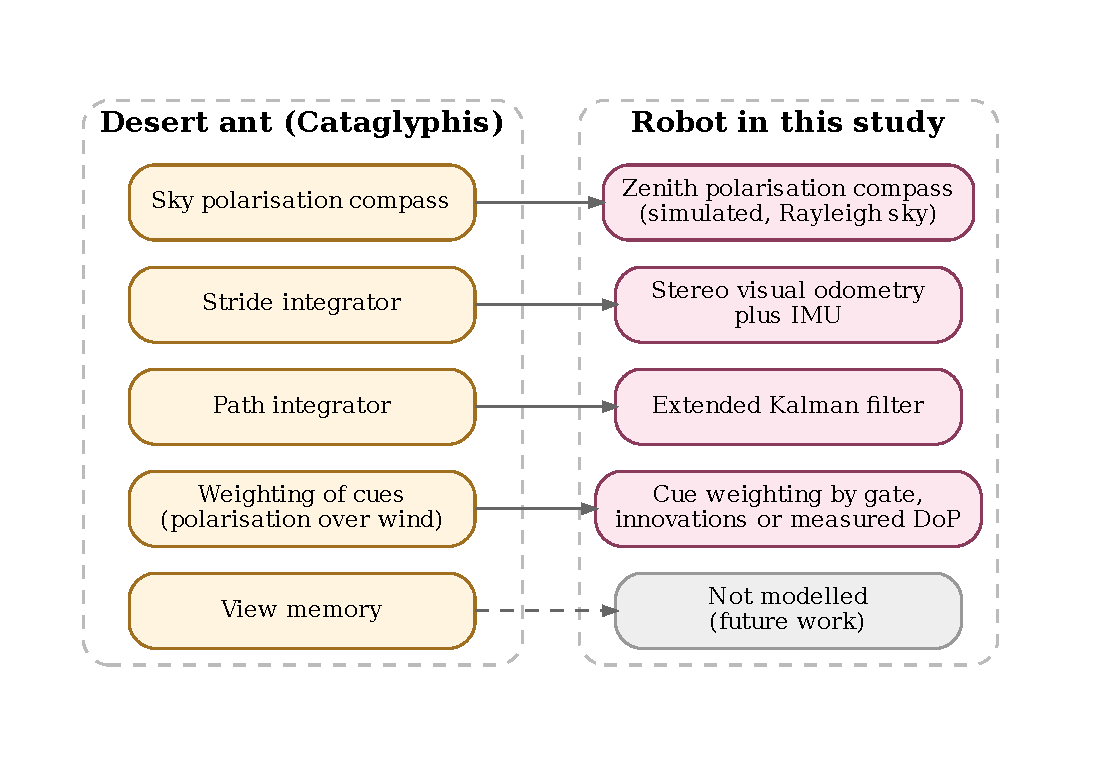
\includegraphics[width=0.7\columnwidth]{diagrams/antmap.pdf}
\caption{Correspondence between the desert ant navigation toolkit and the components studied here. View memory is not modelled.}
\label{fig:antmap}
\end{figure}

\section{Background and Related Work}
\subsection{Insect inspired navigation}
The ant toolkit comprises a skylight polarisation compass, a path integrator and view based place recognition \cite{wehner03}, and the polarisation compass outcompetes the wind compass when available \cite{muller07}. Sahabot, a mobile robot with three polarisation opponent sensors, was reported to navigate with precision comparable to the ant, and its orientation precision dropped sharply when the compass was replaced by proprioception \cite{lambrinos, labhart}. AntBot combined a polarised light compass with optic flow and reported a mean homing error of 0.67 percent \cite{antbot}. Recent work pairs odometry with learned views to cancel drift \cite{gattaux, firlefyn}.

\subsection{Skylight polarisation as a compass}
In the single scattering Rayleigh model the e vector (electric field vector) of skylight is perpendicular to the scattering plane \cite{suhai}, and the degree of linear polarisation (DoP) is $d = d_{\max}\sin^2\gamma/(1+\cos^2\gamma)$ with $\gamma$ the scattering angle \cite{liang}. A full sky study found the measured angle of polarisation within 5 degrees of the Rayleigh model over 13 to 69 percent of the clear sky area \cite{suhai}. In Tunisian desert habitats the clear sky DoP never exceeded a mean of 60 percent, and the DoP is much more affected by atmospheric disturbance than the angle \cite{horvath}. Under clouds the clear sky angle pattern continues where the clouds are lit by the sun, while the DoP is strongly reduced \cite{pomozi}; animals may need only 5 to 10 percent DoP \cite{pomozi}. Measured zenith DoP in the Tunisian desert fell from 24 to 30 percent at a solar elevation of 35 degrees to about 8 percent at 70 degrees \cite{horvath}, and simulations of a desert site with moderate aerosol keep the DoP below 60 percent for most wavelengths \cite{pust}. Lower DoP means larger angle error \cite{ma15}. Near the zenith the sun vector projection vanishes and yaw cannot be estimated when the sun is at the zenith \cite{liang20b, hu22}. Engineered sensors report about 0.5 degrees of dynamic heading deviation against an inertial reference \cite{wang19}, sub degree RMS yaw error on a road vehicle under mostly clear skies \cite{potter}, and 2.82 degrees yaw RMSE in a dynamic inertial and polarisation test \cite{hu22}. Sensor tilt adds errors that grow with tilt and solar altitude \cite{liang}.

\subsection{Heading in visual inertial estimation}
Visual inertial estimators \cite{mourikis, openvins, vinsmono, orbslam3} have no global heading reference, and standard linearised filters gain spurious yaw information that makes them overconfident in yaw and then in position \cite{hesch, huang_fej, limourikis}. Because trajectory alignment usually removes yaw \cite{zhang18}, and a heading aid makes yaw observable, we report drift without alignment as the primary metric, with relative error as a secondary one \cite{sturm, geiger}.

\subsection{Adaptive weighting of a heading aid}
Covariance matching raises the noise estimate when the sample covariance of the innovations exceeds its theoretical value \cite{zhang20}; the identifiability of the full noise matrix under such schemes is disputed \cite{zhang20}. AMO-HEAD inflates a magnetometer noise covariance with chi square tests tuned in the test environment \cite{amohead}. For polarisation compasses specifically, an inertial and polarisation system for ships uses upper and lower DoP thresholds to give the compass full weight, blend its noise, or switch it out \cite{zhang22}; a further scheme cited in \cite{sun25} uses the DoP as a deterministic factor to scale the measurement noise; and other designs adapt the noise statistically by variational Bayes or innovation saturation without a camera \cite{zhao, sun25}. A polarisation compass has been added to a visual inertial filter on a micro aerial vehicle, removing yaw drift \cite{steidle}, and to monocular visual inertial navigation on a road vehicle, improving heading accuracy by 23.4 percent over 2 km \cite{chu23}. Sun-BCNN feeds a learned sun direction with its own uncertainty into stereo visual odometry \cite{sunbcnn}, and magnetometer residuals have been added to visual inertial SLAM \cite{joshi}.

\subsection{Degradation and datasets}
Image corruption benchmarks grade severity in five levels \cite{imagenetc}, but severity orders parameters, not difficulty, and proxy fidelity can change method rankings \cite{failuredrift}. Quantitative studies of dust on cameras for visual odometry are scarce; airborne dust is described as creating non repeatable features \cite{khattak}. Haze is commonly modelled by Koschmieder's law, with radiance attenuated as $e^{-kd}$ and replaced by airlight \cite{cheng}. TartanAir notes that dark scenes are poorly simulated \cite{tartanair}; TartanGround provides 878 ground robot trajectories in 63 environments with stereo, depth and IMU \cite{tartanground}, released under CC BY 4.0 \cite{tg_hf}.

\section{Sky Compass Model}
\label{sec:sky}
The sun position follows the NOAA general solar position equations \cite{noaa} for Abu Dhabi (24.45 N, 54.38 E, UTC+4); its solar zenith angle agrees with an independent implementation (the astral Python package) to within 0.2 degrees at seven reference times recorded in the unit tests. For a zenith view the scattering angle equals the solar zenith angle $\theta_s$, so the zenith DoP is $d = d_{\max}\sin^2\theta_s/(1+\cos^2\theta_s)$ with $d_{\max}=0.6$ \cite{horvath, liang}. The zenith e vector is perpendicular to the solar meridian, so the compass measures heading modulo 180 degrees; the filter resolves the ambiguity with its prior. The angle noise grows as the DoP falls,
\begin{equation}
\sigma_\alpha^2 = \sigma_f^2 + (c/d)^2,\quad \sigma_f = 0.5^\circ,\ c = 0.05^\circ ,
\label{eq:sigma}
\end{equation}
where the floor reflects reported dynamic accuracy \cite{wang19, potter} and the second term is photon limited noise on the Stokes parameters. The sensor also reports a measured DoP with noise 0.002. Sky conditions scale the DoP: clear 1.0, haze 0.6, dust 0.3, and broken cloud, where Markov cloud epochs over the zenith (35 percent of the time, mean 30 s) draw the DoP scale from 0.05 to 0.3 for each sample and add zero mean angle noise of 10 degrees standard deviation, consistent with an angle pattern that persists under cloud while the DoP collapses \cite{pomozi}. The scaling factors are assumptions, not measurements.

Fig.~\ref{fig:sky} shows the consequence. On 21 June the sun passes about 1 degree from the zenith at 12:24 local time, the zenith DoP falls to nearly zero, and the model compass noise exceeds 10 degrees for 64 minutes (11:52 to 12:55) and 2 degrees for 146 minutes. Over the year (a model analysis added after the protocol), the model predicts a period with noise above 10 degrees on 89 days, from 9 May to 5 August, lasting up to 65 minutes. On 21 December and at the equinoxes the noon sun stays at least 23 degrees from the zenith and the compass is usable all day. This blind window follows directly from the latitude of the Gulf being close to the Tropic of Cancer; a polarisation compass that looks at the zenith alone needs another heading source around summer noon.

\begin{figure*}[t]
\centering
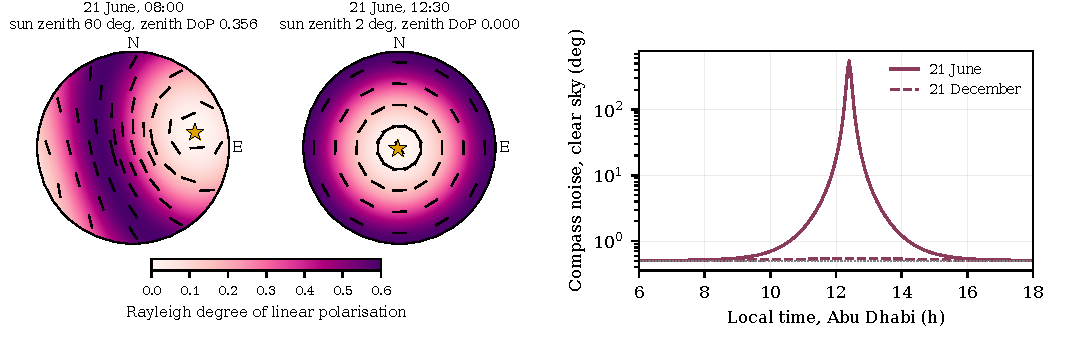
\includegraphics[width=\textwidth]{figs/fig_sky.pdf}
\caption{Sky compass model over Abu Dhabi. Left: Rayleigh DoP over the sky with e vectors (black) and the sun (star) at 08:00 and 12:30 on 21 June; north up, east right, zenith at the centre. Right: model compass noise (\ref{eq:sigma}) for a clear sky through the day.}
\label{fig:sky}
\end{figure*}

\section{System}
\label{sec:system}
Fig.~\ref{fig:arch} shows the pipeline.

\begin{figure*}[t]
\centering
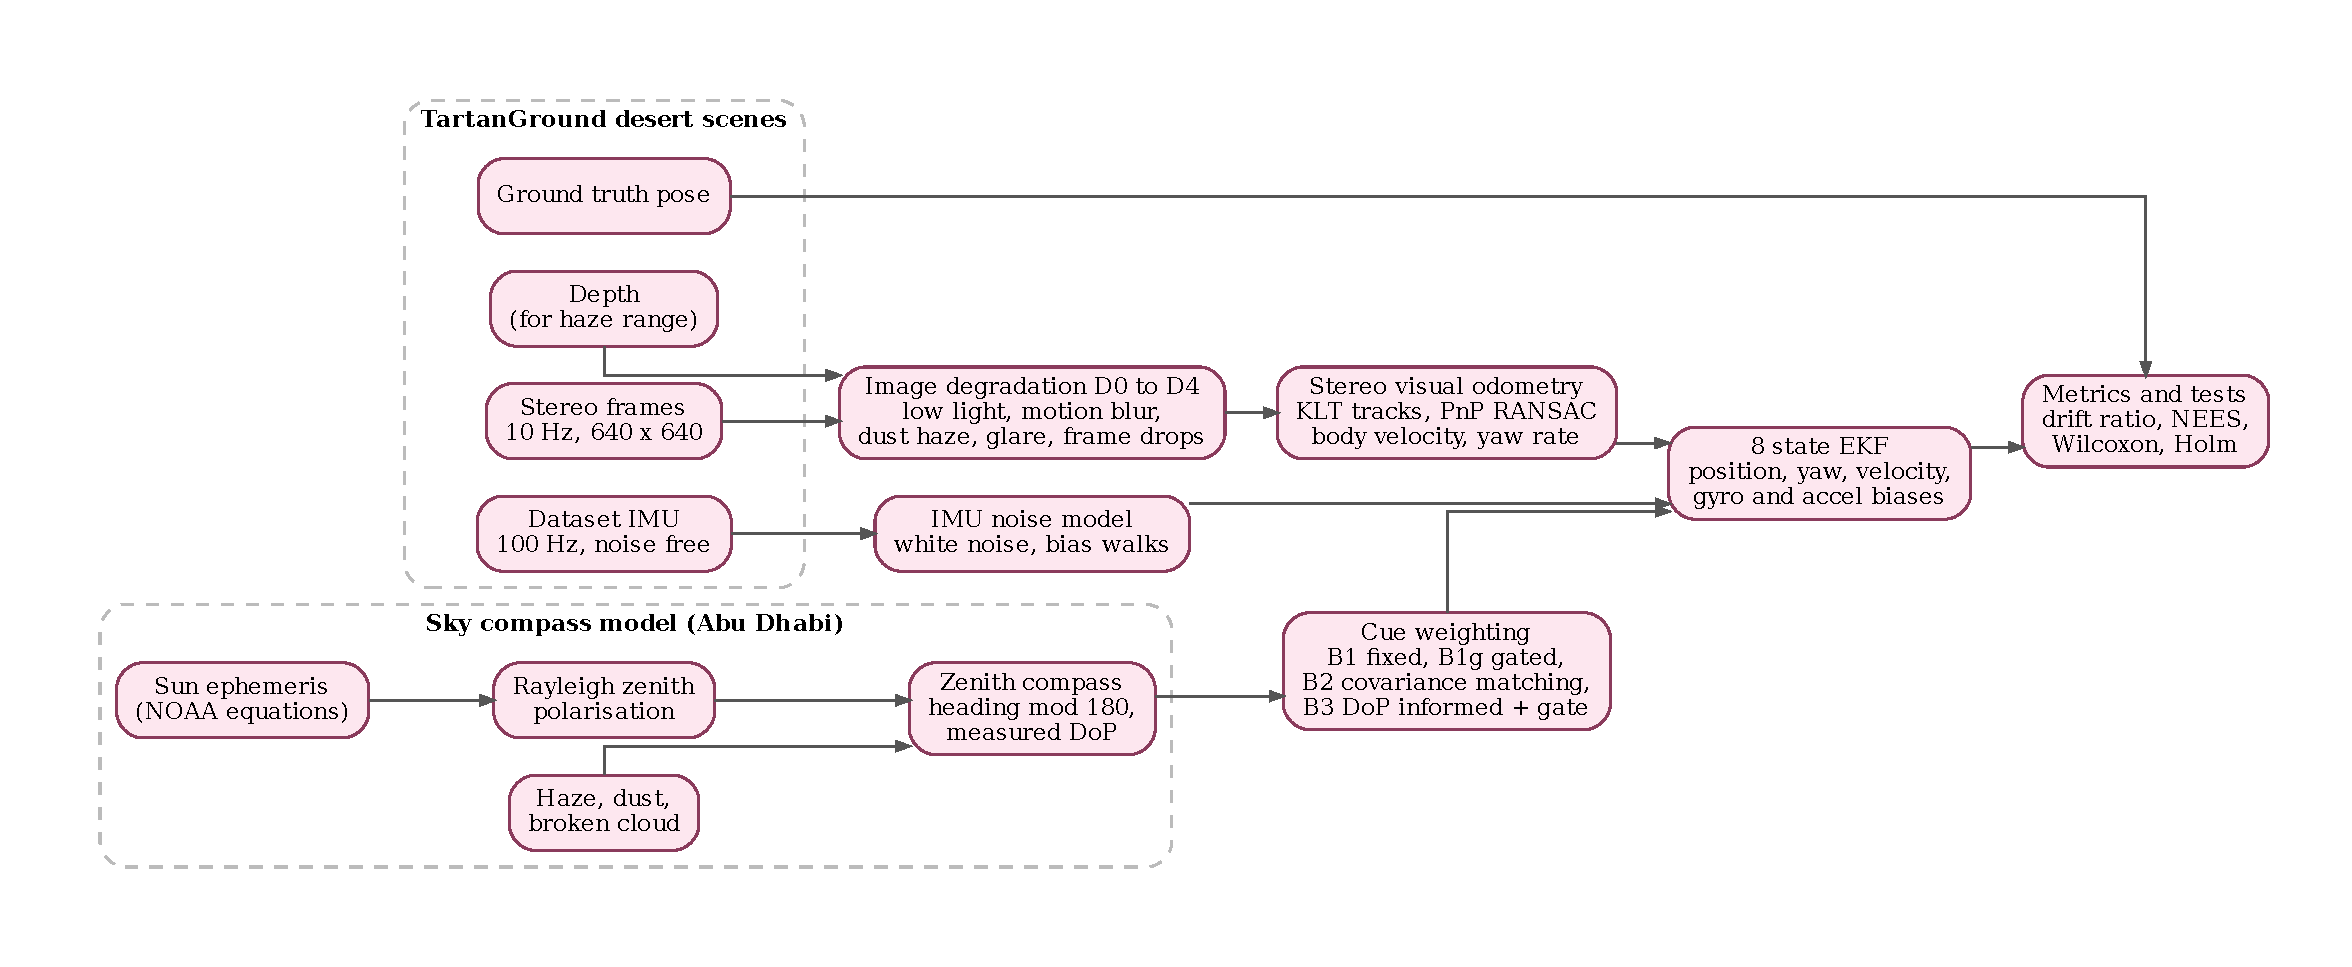
\includegraphics[width=0.85\textwidth]{diagrams/architecture.pdf}
\caption{Study 2 pipeline. Rendered stereo frames are degraded and passed to stereo visual odometry; the IMU receives a noise model; the sky compass model provides heading modulo 180 degrees with a measured DoP; five compass weighting schemes and the no compass baseline share one filter.}
\label{fig:arch}
\end{figure*}

\subsection{Data}
We use TartanGround desert scenes \cite{tartanground}: WesternDesertTown (6 trajectories) as the pilot split and DesertGasStation, MiddleEast and EndofTheWorld (34 trajectories, omni wheeled and differential drive) as the held out split. One held out trajectory used to debug the code before the pilot was excluded. Each trajectory provides the front stereo pair (baseline 0.25 m, 90 degree field of view, 10 Hz), left depth, a 100 Hz IMU and ground truth poses. We keep up to 200 s per trajectory and convert the images to 320 by 320 grayscale. The filter uses the dataset's gravity free body acceleration (forward and right) and the vertical gyro only. Each held out trajectory has one degradation seed per level and two IMU noise draws, shared by all 48 sky scenarios, so B0 has two distinct runs per trajectory and level and the compass systems differ across scenarios through the compass only. The TartanAir documentation describes its IMU as derived from the pose spline without noise \cite{tartanair}, and we treat the TartanGround IMU the same way: we add white noise and bias random walks (gyro 0.002 rad/s$/\sqrt{\mathrm{Hz}}$, accelerometer 0.02 m/s$^2/\sqrt{\mathrm{Hz}}$).

\subsection{Image degradation}
Degradation is applied in linear intensity in the order of image formation: dust haze by Koschmieder attenuation along the rendered depth with airlight \cite{cheng}; a veiling glare with one centre per sequence; auto exposure that lengthens the exposure up to 20 ms and then loses light; motion blur from yaw rate and exposure; photon and read noise; gamma encoding and quantisation; and Markov frame drops. D0 leaves the rendered image unchanged. Levels D1 to D4 set the light gain (0.5 to 0.025), the visibility (1000, 200, 60 and 20 m with the 2 percent contrast convention, $\beta = 3.912/V$; equivalently 766, 153, 46 and 15 m at the 5 percent threshold \cite{cheng}), an additive glare of 0.02 to 0.20 times a glare map, and frame drops of 2 to 20 percent. Fig.~\ref{fig:frames} shows one pilot frame at each level.

\begin{figure*}[t]
\centering
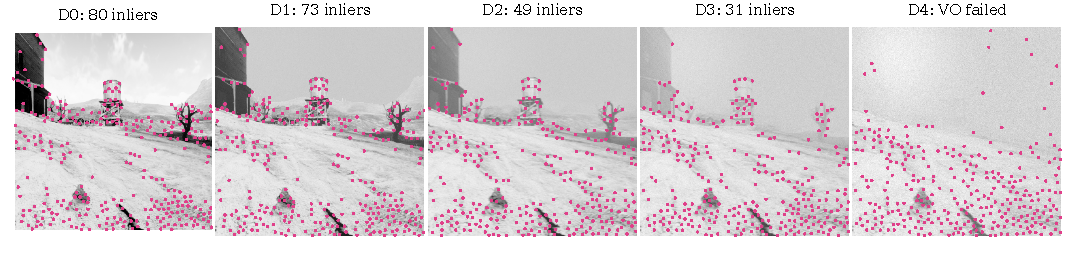
\includegraphics[width=0.9\textwidth]{figs/fig_frames.pdf}
\caption{One pilot frame at levels D0 to D4 with the tracked and newly detected features (dots) and the number of PnP inliers for the step from the previous frame.}
\label{fig:frames}
\end{figure*}

\subsection{Stereo visual odometry}
Features are tracked with pyramidal Lucas Kanade and a forward backward check, triangulated from left right disparity, and the relative pose is solved with PnP and RANSAC. The output per frame is the body velocity (forward, right) and the yaw rate, or a failure flag below 15 inliers. There is no mapping and no loop closure.

\subsection{Filter and weighting schemes}
An eight state extended Kalman filter estimates position, yaw, world velocity, gyro bias and two accelerometer biases. The IMU drives the prediction at 100 Hz; visual odometry updates body velocity and gyro bias at 10 Hz. A visual update whose normalised innovation squared (NIS) exceeds the 99 percent chi square value is kept with its noise multiplied by the ratio of the NIS to that value, which bounds outlier influence without locking the filter out. The compass updates yaw at 5 Hz. The six systems differ only in the compass update: \textbf{B0} no compass; \textbf{B1} fixed noise of 1 degree; \textbf{B1g} fixed noise with a 99 percent chi square gate; \textbf{B2} covariance matching over three innovations as in Study~1, here with a 1 degree floor; \textbf{B3} noise from the measured DoP through (\ref{eq:sigma}) with the same gate; \textbf{B3a} B3 plus a visual noise scale adapted from the mean visual NIS over the last ten updates.

\section{Protocol}
\label{sec:protocol}
Both studies follow the same rules: the primary metric, the statistics and the split are written down and frozen in a repository tag before any held out run; parameters are set on a pilot split only; all runs are reported; deviations are logged \cite{nosek}. This is a self imposed freeze recorded in version control, not an entry in a public registry. Fig.~\ref{fig:protocol} summarises the sequence.

\begin{figure}[t]
\centering
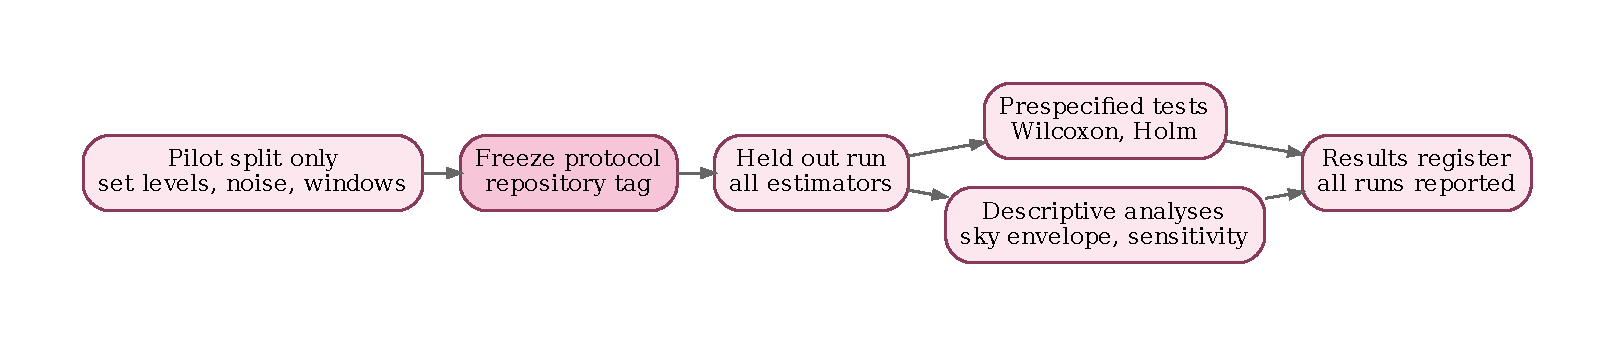
\includegraphics[width=0.9\columnwidth]{diagrams/protocol.pdf}
\caption{Sequence followed in both studies.}
\label{fig:protocol}
\end{figure}

\subsection{Study 1 (surrogate, frozen as protocol v0.1)}
Study~1 used planar synthetic trajectories, a six state filter, a surrogate visual front end (speed and yaw rate measurements whose noise, dropout and outliers grew with the level) and a synthetic heading cue with contamination epochs of 20 to 60 degrees; four systems (B0, B1, B1g, B2) were compared on 24 held out trajectories with 10 seeds each.

\subsection{Study 2 (image based, frozen as protocol v0.2)}
The pilot split set three things: the level parameters (kept after one check that they were graded and not saturated), the nominal visual noise (1.4826 times the median absolute deviation of the D0 visual errors: 0.055 and 0.041 m/s and 0.0049 rad/s), and the B3a window (ten updates, by a written rule). Two pilot fixes were made before the freeze: the initial velocity, set from the first two ground truth poses, received a variance of 4 (m/s) squared, and bounded inflation instead of rejection for visual outliers, after rejection locked the filter out. Each held out visual odometry run is filtered under 48 sky scenarios (21 June and 21 December; start times 07:30, 09:30, 11:45, 12:30, 14:30 and 16:30; clear, haze, dust and broken cloud) with 2 filter seeds.

\textbf{Metrics.} The primary metric is the drift ratio, the final position error divided by the path length, in percent, with no alignment and a known start pose. Tables and figures report trajectory level medians (the median over trajectories of the per trajectory mean), the unit of the tests, unless they say otherwise. Because the compass acts on heading first and the trajectories last at most 200 s, heading RMSE is a second primary metric. Secondary metrics are position RMSE, ATE after SE(2) alignment, relative error over 10 s, failure rate (drift above 10 percent), the median over runs of the time averaged position normalised estimation error squared (NEES, ideal 2) and the mean coverage of the 95 percent position ellipse.

\textbf{Statistics.} The unit of analysis is the trajectory: each metric is averaged over the 96 runs per trajectory, level and system, following the practice of averaging repeated executions per problem \cite{derrac}; runs on the same trajectory share the visual odometry and IMU draws and are not independent. Family F1 tests B3 against B1g, B2 and B0 on drift at each level (15 tests); family F2 tests the same pairs on heading RMSE (15 tests); family F3 tests B3a against B3 on drift and coverage (10 tests). Each test is a paired Wilcoxon signed rank test; we report the median paired difference with a bootstrap 95 percent interval (10,000 resamples \cite{colas}) and the paired dominance delta (share of trajectories with a positive difference minus share with a negative one), with Holm correction within each family \cite{derrac}. Hypotheses written before the run: H1, B3 beats B0 on drift and heading at D2 to D4; H2, B3 beats B1g on heading because of the near noon June scenarios; H3, B3 is not worse than B2 (no non inferiority margin was set, so H3 is judged by two sided tests); H4, B3a beats B3 on drift and coverage.

\section{Results}
\label{sec:results}
\subsection{Study 1: surrogate study}
On 24 held out synthetic trajectories, any heading cue lowered the drift once the surrogate vision degraded: at the middle level the run level median drift fell from 5.12 percent of path length (B0) to 1.20 percent (B1g and B2). Covariance matching (B2) beat the ungated cue (B1) at four of five levels, but was indistinguishable from the gated cue (B1g) at every level, with confidence intervals of the paired difference within 0.05 percentage points. A descriptive sensitivity grid at the middle level showed that the gate fails when the true cue noise is several times the assumed value (run level medians at 16 degrees: 4.51 percent for B1g, 1.94 for B2 and 1.99 for B1) and that a cue bias random walk of 2 degrees per $\sqrt{\mathrm{s}}$ made every heading aided system worse than B0. Every filter was overconfident. Study~1 therefore pointed to a cue whose reliability varies for a physical reason, and to a weighting that follows that reason, which Study~2 tests.

\subsection{Study 2: visual odometry under degradation}
On the held out split, the median share of frames with a valid visual odometry estimate fell from \nvoOkDzero{} at D0 to \nvoOkDfour{} at D4, and the robust yaw rate error rose from \nvoSigWDzero{} to \nvoSigWDfour{} rad/s, so the levels are graded and D4 is severe but not saturated. Study~2 comprises \nnTraj{} trajectories, \nnRunsCell{} runs per system and level, and \nnRuns{} filter runs in total.

\subsection{Study 2: drift and heading}
Table~\ref{tab:e02main} and Fig.~\ref{fig:e02main} give the trajectory level medians. Without a compass, the heading RMSE grows from \nthdBzerozero{} degrees at D0 to \nthdBzerofour{} degrees at D4 and the drift from \ntdrBzerozero{} to \ntdrBzerofour{} percent of path length.

The ungated fixed weight compass B1 is worse than no compass on drift at every level (\ntdrBoneone{} to \ntdrBonefour{} percent) and on heading at D0 to D3 (\nthdBonezero{} to \nthdBonethree{} degrees against \nthdBzerozero{} to \nthdBzerothree{}); at D4 its heading RMSE (\nthdBonefour{}) is below that of B0 (\nthdBzerofour{}). The cause is a few runs at 12:30 on 21 June that fail badly (Section~\ref{sec:tod}). Outside the June noon window (excluding the 11:45 and 12:30 June scenarios, a descriptive cut) its heading RMSE is \nowhdBonezero{} to \nowhdBonetwo{} degrees, competitive with the weighted schemes at D2 to D4 but not at D0.

The four weighted schemes (B1g, B2, B3 and B3a) keep the heading RMSE between \nthdBtwozero{} and \nthdBgatefour{} degrees. At D3 and D4 they reduce the heading RMSE by a factor of \nhratioMinthree{} to \nhratioMaxfour{} and the drift by \ndredMinthree{} to \ndredMaxfour{} percent relative to B0. We expect, without having tested it, that the remaining drift comes mostly from visual odometry translation errors, which a heading aid cannot correct. The secondary metrics agree: at D3 the run level median ATE after SE(2) alignment is \nateBzerothree{} m for B0 and \nateBthreethree{} m for B3, and the relative error over 10 s is \nrpeBzerothree{} m against \nrpeBthreethree{} m.

\begin{table}[t]
\caption{Study 2 held out results. Drift and heading: trajectory level medians ($n=\nnTraj$). Failure: share of the \nnRunsCell{} runs per cell with drift above 10 percent.}
\label{tab:e02main}
\centering\footnotesize\setlength{\tabcolsep}{4pt}
\begin{tabular}{lrrrrrr}
\toprule
Level & B0 & B1 & B1g & B2 & B3 & B3a \\
\midrule
\multicolumn{7}{l}{\emph{Drift ratio (\%), trajectory level}} \\
D0 & 0.92 & 3.06 & 0.91 & 0.87 & 0.88 & 0.90 \\
D1 & 1.52 & 3.04 & 1.10 & 1.00 & 1.03 & 0.99 \\
D2 & 1.90 & 3.10 & 1.45 & 1.22 & 1.37 & 1.29 \\
D3 & 2.60 & 3.90 & 1.96 & 1.54 & 1.73 & 1.76 \\
D4 & 5.00 & 5.16 & 3.04 & 3.19 & 3.26 & 2.61 \\
\midrule
\multicolumn{7}{l}{\emph{Heading RMSE (deg), trajectory level}} \\
D0 & 1.68 & 6.68 & 0.67 & 0.49 & 0.53 & 0.55 \\
D1 & 2.84 & 7.20 & 0.93 & 0.70 & 0.74 & 0.69 \\
D2 & 3.68 & 7.60 & 1.36 & 0.85 & 0.98 & 0.91 \\
D3 & 7.66 & 7.95 & 1.93 & 1.49 & 1.61 & 1.37 \\
D4 & 9.29 & 8.41 & 2.33 & 1.46 & 1.78 & 1.72 \\
\midrule
\multicolumn{7}{l}{\emph{Failure rate (share of runs with drift above 10\%)}} \\
D0 & 0.00 & 0.07 & 0.00 & 0.00 & 0.00 & 0.00 \\
D1 & 0.00 & 0.07 & 0.00 & 0.00 & 0.00 & 0.00 \\
D2 & 0.03 & 0.07 & 0.01 & 0.00 & 0.00 & 0.00 \\
D3 & 0.09 & 0.10 & 0.05 & 0.03 & 0.04 & 0.05 \\
D4 & 0.16 & 0.17 & 0.11 & 0.11 & 0.11 & 0.11 \\
\bottomrule
\end{tabular}
\end{table}

\begin{figure*}[t]
\centering
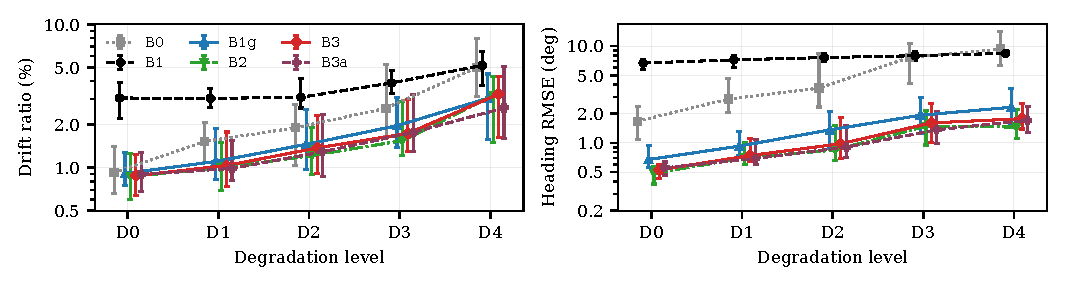
\includegraphics[width=\textwidth]{figs/fig_e02_main.pdf}
\caption{Study 2 held out results by degradation level: trajectory level median drift (left) and heading RMSE (right) with interquartile range over the \nnTraj{} trajectories, logarithmic axes.}
\label{fig:e02main}
\end{figure*}

\subsection{Study 2: prespecified tests}
Table~\ref{tab:e02tests} gives families F1 and F2 ($n=\nnTraj$). \textbf{H1} is supported: B3 has lower drift than B0 at D1 to D4 (Holm adjusted $p \le$ \nFonetwoBzerop{}; at D2 the bootstrap interval of the median difference, [\nFonetwoBzerolo{}, \nFonetwoBzerohi{}], includes zero; at D0 the adjusted $p$ is \nFonezeroBzerop{}) and lower heading RMSE at every level. \textbf{H2} is supported in direction: B3 has lower heading RMSE than the gated fixed weight B1g at every level, by 0.14 to 0.37 degrees, and family F1 shows lower drift as well. Its stated reason, the near noon scenarios, is only part of the story: descriptively, B3 also beats B1g outside the noon window at D0 to D3, by \nowgapMin{} to \nowgapMax{} degrees in the paired trajectory median. \textbf{H3} is rejected: B2 is slightly but consistently better than B3, by \nFoneoneBtwodiff{} to \nFonefourBtwodiff{} percentage points of drift at D1 to D4 and by \nFtwozeroBtwodiff{} to \nFtwofourBtwodiff{} degrees of heading RMSE, all significant after Holm correction. \textbf{H4} is half supported: B3a does not change the drift (all adjusted $p = 1$) but raises the 95 percent coverage at D1 to D4 (adjusted $p \le$ \nFthreefourcoverp{}), for example at D4 from a trajectory median of \nFthreefourcoverB{} to \nFthreefourcoverA{}, still far below 0.95. B2 and B1g were not compared in a prespecified family; descriptively, B2 has lower heading RMSE than B1g at every level (uncorrected Wilcoxon $p < 0.001$).

\begin{table}[t]
\caption{Study 2 prespecified paired tests of B3 against each baseline, trajectory level ($n=\nnTraj$). Diff is B3 minus the baseline (negative favours B3). $\delta$ is the paired dominance delta.}
\label{tab:e02tests}
\centering\footnotesize\setlength{\tabcolsep}{3.5pt}
\begin{tabular}{llrrrr}
\toprule
Level & Pair & Diff & 95\% CI & $\delta$ & $p_{\mathrm{Holm}}$ \\
\midrule
\multicolumn{6}{l}{\emph{F1: drift ratio (percentage points)}} \\
D0 & B3 vs B1g & -0.05 & [-0.07, -0.02] & -0.59 & $<$0.001 \\
 & B3 vs B2 & 0.01 & [0.00, 0.02] & 0.18 & 0.063 \\
 & B3 vs B0 & -0.09 & [-0.15, 0.00] & -0.35 & 0.063 \\
D1 & B3 vs B1g & -0.06 & [-0.10, -0.03] & -0.76 & $<$0.001 \\
 & B3 vs B2 & 0.03 & [0.02, 0.06] & 0.82 & $<$0.001 \\
 & B3 vs B0 & -0.52 & [-0.77, -0.23] & -0.65 & $<$0.001 \\
D2 & B3 vs B1g & -0.08 & [-0.16, -0.06] & -0.82 & $<$0.001 \\
 & B3 vs B2 & 0.03 & [0.01, 0.06] & 0.76 & $<$0.001 \\
 & B3 vs B0 & -0.25 & [-0.95, 0.05] & -0.24 & 0.018 \\
D3 & B3 vs B1g & -0.11 & [-0.18, -0.06] & -0.76 & $<$0.001 \\
 & B3 vs B2 & 0.04 & [0.02, 0.08] & 0.76 & $<$0.001 \\
 & B3 vs B0 & -0.98 & [-1.66, -0.20] & -0.47 & $<$0.001 \\
D4 & B3 vs B1g & -0.11 & [-0.19, -0.02] & -0.47 & 0.015 \\
 & B3 vs B2 & 0.09 & [0.03, 0.13] & 0.47 & 0.003 \\
 & B3 vs B0 & -1.68 & [-2.67, -0.58] & -0.59 & $<$0.001 \\
\midrule
\multicolumn{6}{l}{\emph{F2: heading RMSE (deg)}} \\
D0 & B3 vs B1g & -0.14 & [-0.17, -0.12] & -0.88 & $<$0.001 \\
 & B3 vs B2 & 0.04 & [0.03, 0.07] & 0.76 & $<$0.001 \\
 & B3 vs B0 & -1.06 & [-1.52, -0.74] & -1.00 & $<$0.001 \\
D1 & B3 vs B1g & -0.17 & [-0.29, -0.13] & -0.82 & $<$0.001 \\
 & B3 vs B2 & 0.04 & [0.02, 0.10] & 0.47 & $<$0.001 \\
 & B3 vs B0 & -2.00 & [-3.25, -1.63] & -0.94 & $<$0.001 \\
D2 & B3 vs B1g & -0.23 & [-0.41, -0.17] & -0.76 & $<$0.001 \\
 & B3 vs B2 & 0.07 & [0.05, 0.17] & 0.82 & $<$0.001 \\
 & B3 vs B0 & -2.79 & [-3.78, -1.77] & -1.00 & $<$0.001 \\
D3 & B3 vs B1g & -0.33 & [-0.59, -0.26] & -0.88 & $<$0.001 \\
 & B3 vs B2 & 0.15 & [0.08, 0.22] & 0.76 & $<$0.001 \\
 & B3 vs B0 & -6.00 & [-7.67, -3.30] & -0.94 & $<$0.001 \\
D4 & B3 vs B1g & -0.37 & [-0.60, -0.14] & -0.59 & $<$0.001 \\
 & B3 vs B2 & 0.38 & [0.20, 0.50] & 0.88 & $<$0.001 \\
 & B3 vs B0 & -7.48 & [-10.58, -6.31] & -1.00 & $<$0.001 \\
\bottomrule
\end{tabular}
\end{table}

\subsection{Study 2: time of day and sky condition}
\label{sec:tod}
Fig.~\ref{fig:envelope} shows mean heading RMSE by start time and sky on 21 June (descriptive, as prespecified). The ungated fixed weight B1 is the best or joint best system at most times in clear, hazy and dusty skies (under cloud B2 is best), but when the sun is nearest the zenith it fails: at 12:30 its mean heading RMSE is \nhnoonBone{} degrees and its mean drift \ndnoonBone{} percent, against \nhnoonBzero{} degrees and \ndnoonBzero{} percent for B0. Fig.~\ref{fig:traj} shows one such held out run. All weighted schemes fall back to roughly the B0 level at 12:30 (\nhnoonBgate{}, \nhnoonBtwo{}, \nhnoonBthree{} and \nhnoonBthreea{} degrees for B1g, B2, B3 and B3a), the correct behaviour for a blind sensor. At 11:45, when the compass is degraded but still informative, the gate alone discards most of it (B1g \nhnearBgate{} degrees), while B3 (\nhnearBthree{}) and B3a (\nhnearBthreea{}) do better than B2 (\nhnearBtwo{}). On 21 December there is no blind window and all compass systems stay below one degree on average (B1 \nhdecBone{}, B2 \nhdecBtwo{}, B3 \nhdecBthree{}).

Broken cloud is where B3 loses to B2: over all cloud scenarios its mean heading RMSE is \nskycloudBthree{} degrees against \nskycloudBtwo{} for B2. The gated systems reject far more compass samples under cloud (per run, B1g \ngatedcloudBgate{} under cloud against \ngatedotherBgate{} otherwise; B3 \ngatedcloudBthree{} against \ngatedotherBthree{}), and in an analysis added after the run, \nstuckBthree{} percent of B3 and \nstuckBgate{} percent of B1g cloud runs outside the noon window ended with a heading error above 3 degrees, against \nstuckBtwo{} percent for B2 and \nstuckBone{} percent for B1. This pattern is consistent with gate lock out: a cloud epoch adds angle noise that the measured DoP does not fully reflect, the heading drifts beyond the gate, and later valid samples are rejected. We did not test this mechanism directly.

\begin{figure*}[t]
\centering
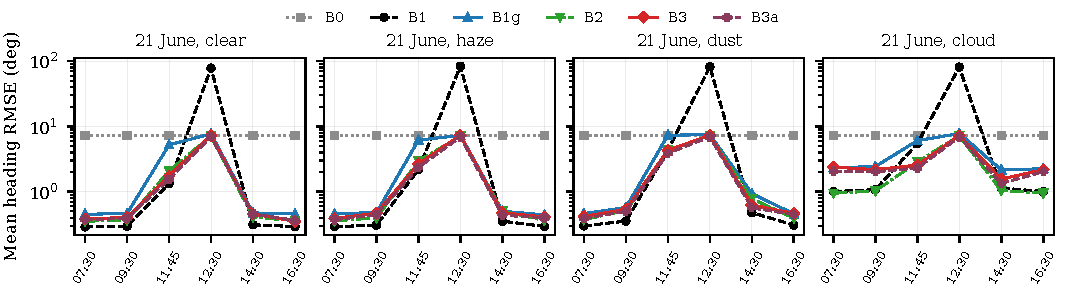
\includegraphics[width=\textwidth]{figs/fig_envelope.pdf}
\caption{Study 2, 21 June: mean heading RMSE by start time for each sky condition, all levels pooled. The ungated fixed weight B1 fails in the noon window; the weighted schemes fall back to the no compass level.}
\label{fig:envelope}
\end{figure*}

\begin{figure*}[t]
\centering
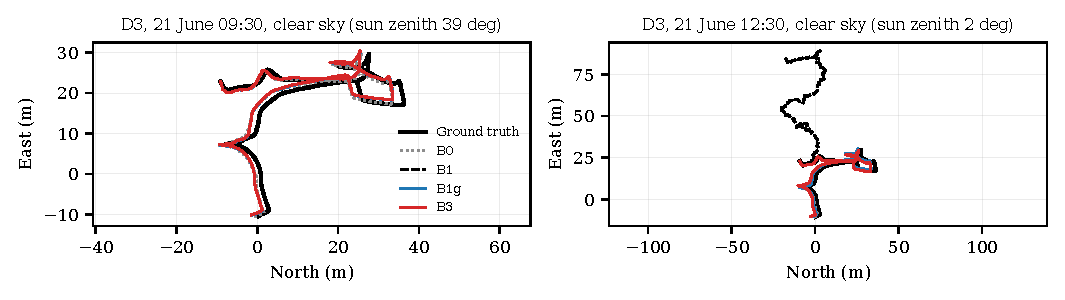
\includegraphics[width=\textwidth]{figs/fig_traj.pdf}
\caption{One held out run (MiddleEast omni wheeled trajectory P0000, level D3, clear sky, 21 June, filter seed 0). Left, 09:30: all systems stay close to the truth on this trajectory (final drift \nexmornBzero{} percent for B0 and \nexmornBthree{} for B3). Right, 12:30: the fixed weight compass B1 diverges (\nexnoonBone{} percent), while B1g and B3 stay close (\nexnoonBgate{} and \nexnoonBthree{} percent).}
\label{fig:traj}
\end{figure*}

\subsection{Study 2: consistency}
No system is consistent. The median position NEES lies between \nneBthreeafour{} and \nneBonethree{} against an ideal of 2, and the mean 95 percent coverage between \ncvBzerothree{} and \ncvBthreeafour{} against 0.95. B3a raises coverage, as reported above. A likely cause of the overconfidence, not tested here, is that the visual odometry errors are biased and correlated in time while the filter treats them as white.

\subsection{Exploratory analysis after the held out run}
The cloud result suggests replacing B3's hard gate with innovation based inflation. We added, after the held out run and outside the prespecified tests, a system B4 that uses the DoP based noise as the floor of covariance matching with no gate. On the same held out runs it ties B2: under cloud its mean heading RMSE is \nskycloudBfour{} degrees against \nskycloudBtwo{}, and its per trajectory mean heading RMSE is lower than that of B2 on \nbfourSharezero{}, \nbfourShareone{}, \nbfourSharetwo{}, \nbfourSharethree{} and \nbfourSharefour{} percent of trajectories at D0 to D4, with trajectory level medians of \nbfourMedfour{} against \nbtwoMedfour{} degrees at D4. This is a hypothesis for a future frozen test, not a finding.

\section{Discussion}
\textbf{Weighting is necessary, and the noon window is the reason.} An ungated fixed weight compass is among the best systems for much of the day and the worst system when the sun is nearest the zenith, where it is far worse than having no compass; averaged over the day it is worse than no compass on drift. At Gulf latitude this window recurs on many days of the year, so a deployment needs a reliability mechanism. In our results a hard gate alone discards useful information when the sky is partly informative (11:45), weighting by the measured DoP extracts more of that partial information than the other weighting schemes, and innovation based covariance matching is slightly better over the whole day, with the gate the likely weak point under broken cloud.

\textbf{The filter covariance is not usable downstream.} Drift and heading improve, but no filter reports its own uncertainty honestly: in Study~2 the mean coverage of the 95 percent ellipse lies between \ncvBzerothree{} and \ncvBthreeafour{}, and Study~1 showed the same overconfidence. The visual noise in the filter is fixed at its clear image value while the true visual error grows with the level, and the visual errors are likely biased and correlated in time, so the predicted covariance shrinks faster than the error. A path planner or safety monitor that trusted this covariance would be misled exactly when vision degrades. The same overconfidence weakens every scheme that compares an innovation with its predicted covariance, a chi square gate and covariance matching alike, which is consistent with the gate rejections we observed under cloud. Adapting the visual noise (B3a) raised coverage but did not close the gap.

\textbf{Relation to Study 1.} Study~1 isolated the information a heading cue adds, without a visual front end to confound the statistics, and found that innovation based adaptation did not beat a gate under a synthetic contamination model. Study~2, with a cue whose reliability varies for a physical reason, finds descriptively that covariance matching does beat the gate. Both studies are consistent with the gate being fragile when the cue noise departs from its nominal value.

\subsection*{Threats to validity}
\emph{Rendered and simulated evidence.} Scenes are rendered, not photographed; the scene lighting does not match the compass scenario's sun; the compass is simulated with assumed sky factors. \emph{B3 is matched to the simulator.} B3 uses the same noise law and constants that generate the compass error, which favours it; only the cloud term is unmodelled. The simulated compass error is white, with no bias and no tilt, while Study~1 showed that a drifting bias makes a heading aid harmful. \emph{Model of the noon window.} Measured desert zenith DoP at a solar elevation of 70 degrees was about 8 percent \cite{horvath}, against \ndopSeventy{} percent in our model, so the model may overstate the window; in a sensitivity analysis added after the protocol, doubling the zenith DoP shrinks the June window above 10 degrees from \njuneTen{} to \njuneTenDouble{} minutes. Aerosol lowers the DoP \cite{pust}, which would widen it. \emph{Degradation.} The haze model uses the left depth for both cameras and a single airlight; lens soiling is not modelled. \emph{Filter.} The filter is planar, uses the dataset's gravity free acceleration and the vertical gyro, couples visual odometry loosely without mapping, and is overconfident. A full SE(3) visual inertial estimator adds roll and pitch coupling and gravity alignment errors that a planar filter cannot show; repeating the protocol in such an estimator \cite{openvins} is the step between this study and hardware. \emph{Sample.} Trajectories last at most 200 s; each trajectory has one degradation seed and two IMU draws per level, so variation across scenarios comes from the compass only. \emph{Statistics.} The tests are within one rendered dataset and one compass model; the B2 against B1g comparison, the cloud analysis, the yearly window count and B4 carry no inferential weight.

\section{Conclusion}
A zenith sky compass, modelled with the sun over Abu Dhabi, is a strong heading aid for a desert ground robot whose cameras degrade, but in our model it goes blind around solar noon on \nblindDays{} days of the year. In \nnTraj{} held out rendered desert trajectories with five levels of image degradation, an ungated fixed weight compass was worse than none on drift because it failed in that window, a gate discarded useful information near it, weighting by the measured degree of polarisation used that partial information best among the weighting schemes, and covariance matching was slightly better over the whole day. For an engineer the lesson is short: never fuse a sky compass with a fixed weight; a chi square gate is a cheap first defence that captured almost all of the benefit of adaptation in the surrogate study, but when the cue fades gradually, as the sky does near noon or under cloud, weighting by innovations or by the measured DoP is worth its small extra cost. The next steps are a frozen test of DoP weighting without a hard gate, longer trajectories, a compass error model with bias and tilt, and a real polarisation sensor on a rover in the Gulf summer.

\begin{thebibliography}{99}
\bibitem{icao_wp69} IATA, Working Paper 69, MIDANPIRG/21, ICAO. [Online]. Available: \url{https://www.icao.int/Meetings/MIDANPIRG-RASG/Documents/WP\%2069.pdf}
\bibitem{easa_sib} EASA, ``Safety Information Bulletin 2022-02R4: GNSS outages and alterations,'' 3 Jul. 2026.
\bibitem{ukmto} UKMTO, ``Advisory 034-25 and summary report,'' 3--7 Oct. 2025.
\bibitem{mscio} MSCIO, ``Advisory 01/2026, Update 12,'' 2 Apr. 2026.
\bibitem{uae_icao} United Arab Emirates, working paper WP05, 14th Meeting of the MIDANPIRG CNS Sub-Group, ICAO, Oct. 2025.
\bibitem{hesch} J. A. Hesch, D. G. Kottas, S. L. Bowman, and S. I. Roumeliotis, ``Camera-IMU-based localization: Observability analysis and consistency improvement,'' \emph{Int. J. Robot. Res.}, vol. 33, no. 1, pp. 182--201, 2014.
\bibitem{vinsmono} T. Qin, P. Li, and S. Shen, ``VINS-Mono: A robust and versatile monocular visual-inertial state estimator,'' \emph{IEEE Trans. Robot.}, vol. 34, no. 4, 2018.
\bibitem{mer} M. Maimone, Y. Cheng, and L. Matthies, ``Two years of visual odometry on the Mars Exploration Rovers,'' \emph{J. Field Robot.}, vol. 24, no. 3, pp. 169--186, 2007.
\bibitem{madmax} L. Meyer \emph{et al.}, ``The MADMAX data set for visual-inertial rover navigation on Mars,'' \emph{J. Field Robot.}, 2021, doi:10.1002/rob.22016.
\bibitem{ronacher} B. Ronacher, ``Path integration in a three-dimensional world: the case of desert ants,'' \emph{J. Comp. Physiol. A}, vol. 206, no. 3, pp. 379--387, 2020.
\bibitem{wittlinger} M. Wittlinger, R. Wehner, and H. Wolf, ``The ant odometer: stepping on stilts and stumps,'' \emph{Science}, vol. 312, no. 5782, pp. 1965--1967, 2006.
\bibitem{muller88} M. M\"uller and R. Wehner, ``Path integration in desert ants, \emph{Cataglyphis fortis},'' \emph{Proc. Natl. Acad. Sci. USA}, vol. 85, no. 14, pp. 5287--5290, 1988.
\bibitem{sommer04} S. Sommer and R. Wehner, ``The ant's estimation of distance travelled: experiments with desert ants, \emph{Cataglyphis fortis},'' \emph{J. Comp. Physiol. A}, vol. 190, no. 1, pp. 1--6, 2004.
\bibitem{stone} T. Stone \emph{et al.}, ``An anatomically constrained model for path integration in the bee brain,'' \emph{Curr. Biol.}, vol. 27, no. 20, pp. 3069--3085, 2017.
\bibitem{antbot} J. Dupeyroux, J. R. Serres, and S. Viollet, ``AntBot: A six-legged walking robot able to home like desert ants in outdoor environments,'' \emph{Sci. Robot.}, vol. 4, no. 27, eaau0307, 2019.
\bibitem{decroon} G. C. H. E. de Croon, J. J. G. Dupeyroux, S. B. Fuller, and J. A. R. Marshall, ``Insect-inspired AI for autonomous robots,'' \emph{Sci. Robot.}, vol. 7, no. 67, eabl6334, 2022.
\bibitem{wehner03} R. Wehner, ``Desert ant navigation: how miniature brains solve complex tasks,'' \emph{J. Comp. Physiol. A}, vol. 189, no. 8, pp. 579--588, 2003.
\bibitem{muller07} M. M\"uller and R. Wehner, ``Wind and sky as compass cues in desert ant navigation,'' \emph{Naturwissenschaften}, vol. 94, no. 7, pp. 589--594, 2007.
\bibitem{labhart} Labhart Laboratory, ``Mobile robot employing insect strategies for navigation'' (project page). [Online]. Available: \url{https://mls.uzh.ch/en/research/fgrimls/Labhart/ModelsRobots/MobileRobot.html}
\bibitem{lambrinos} D. Lambrinos, R. M\"oller, T. Labhart, R. Pfeifer, and R. Wehner, ``A mobile robot employing insect strategies for navigation,'' \emph{Robot. Auton. Syst.}, vol. 30, no. 1--2, pp. 39--64, 2000.
\bibitem{gattaux} G. G. Gattaux, J. R. Serres, F. Ruffier, and A. Wystrach, ``Visual homing in outdoor robots using mushroom body circuits and learning walks,'' arXiv:2507.09725, 2025.
\bibitem{firlefyn} M. V. M. Firlefyn, J. J. Hagenaars, and G. C. H. E. de Croon, ``Direct learning of home vector direction for insect-inspired robot navigation,'' arXiv:2405.03827, 2024.
\bibitem{horvath} G. Horv\'ath and R. Wehner, ``Skylight polarization as perceived by desert ants and measured by video polarimetry,'' \emph{J. Comp. Physiol. A}, vol. 184, pp. 1--7, 1999.
\bibitem{mourikis} A. I. Mourikis and S. I. Roumeliotis, ``A multi-state constraint Kalman filter for vision-aided inertial navigation,'' in \emph{Proc. IEEE ICRA}, 2007, pp. 3565--3572.
\bibitem{openvins} P. Geneva, K. Eckenhoff, W. Lee, Y. Yang, and G. Huang, ``OpenVINS: A research platform for visual-inertial estimation,'' in \emph{Proc. IEEE ICRA}, 2020, pp. 4666--4672.
\bibitem{orbslam3} C. Campos, R. Elvira, J. J. G\'omez Rodr\'iguez, J. M. M. Montiel, and J. D. Tard\'os, ``ORB-SLAM3: An accurate open-source library for visual, visual-inertial and multi-map SLAM,'' \emph{IEEE Trans. Robot.}, 2021.
\bibitem{huang_fej} G. P. Huang, A. I. Mourikis, and S. I. Roumeliotis, ``A first-estimates Jacobian EKF for improving SLAM consistency,'' in \emph{Experimental Robotics}, Springer, 2009, pp. 373--382.
\bibitem{limourikis} M. Li and A. I. Mourikis, ``High-precision, consistent EKF-based visual-inertial odometry,'' \emph{Int. J. Robot. Res.}, vol. 32, no. 6, pp. 690--711, 2013.
\bibitem{zhang18} Z. Zhang and D. Scaramuzza, ``A tutorial on quantitative trajectory evaluation for visual(-inertial) odometry,'' in \emph{Proc. IEEE/RSJ IROS}, 2018, pp. 7244--7251.
\bibitem{sturm} J. Sturm, N. Engelhard, F. Endres, W. Burgard, and D. Cremers, ``A benchmark for the evaluation of RGB-D SLAM systems,'' in \emph{Proc. IEEE/RSJ IROS}, 2012, pp. 573--580.
\bibitem{geiger} A. Geiger, P. Lenz, and R. Urtasun, ``Are we ready for autonomous driving? The KITTI vision benchmark suite,'' in \emph{Proc. IEEE CVPR}, 2012, pp. 3354--3361.
\bibitem{zhang20} L. Zhang, D. Sidoti, A. Bienkowski, K. R. Pattipati, Y. Bar-Shalom, and D. L. Kleinman, ``On the identification of noise covariances and adaptive Kalman filtering: A new look at a 50 year-old problem,'' \emph{IEEE Access}, vol. 8, pp. 59362--59388, 2020.
\bibitem{amohead} Q. Guo, S. Yang, J. Lyu, J. Sun, D. Lin, and S. He, ``AMO-HEAD: Adaptive MARG-only heading estimation for UAVs under magnetic disturbances,'' arXiv:2510.10979, 2025.
\bibitem{imagenetc} D. Hendrycks and T. Dietterich, ``Benchmarking neural network robustness to common corruptions and perturbations,'' in \emph{Proc. ICLR}, 2019.
\bibitem{failuredrift} A. S. Thomas, S. Agnihotri, and M. Keuper, ``Failure or drift? Evaluating monocular SLAM under synthetic and real-world corruptions,'' arXiv:2608.30690, 2026.
\bibitem{khattak} S. Khattak, C. Papachristos, and K. Alexis, ``Visual-thermal landmarks and inertial fusion for navigation in degraded visual environments,'' arXiv:1903.01656, 2019.
\bibitem{tartanair} W. Wang \emph{et al.}, ``TartanAir: A dataset to push the limits of visual SLAM,'' arXiv:2003.14338, 2020; and TartanAir documentation, \url{https://tartanair.org}.
\bibitem{tartanground} M. Patel \emph{et al.}, ``TartanGround: A large-scale dataset for ground robot perception and navigation,'' arXiv:2505.10696, 2025.
\bibitem{sunbcnn} V. Peretroukhin, L. Clement, and J. Kelly, ``Reducing drift in visual odometry by inferring sun direction using a Bayesian convolutional neural network,'' arXiv:1609.05993, 2016.
\bibitem{joshi} B. Joshi and I. Rekleitis, ``Enhancing visual inertial SLAM with magnetic measurements,'' arXiv:2409.09904, 2024.
\bibitem{zhao} H. Zhao \emph{et al.}, ``Seamless micro-electro-mechanical system-inertial navigation system/polarization compass navigation method with data and model dual-driven approach,'' \emph{Micromachines}, vol. 15, no. 2, p. 237, 2024, doi:10.3390/mi15020237.
\bibitem{nosek} B. A. Nosek, C. R. Ebersole, A. C. DeHaven, and D. T. Mellor, ``The preregistration revolution,'' \emph{Proc. Natl. Acad. Sci. USA}, vol. 115, no. 11, pp. 2600--2606, 2018.
\bibitem{derrac} J. Derrac, S. Garc\'ia, D. Molina, and F. Herrera, ``A practical tutorial on the use of nonparametric statistical tests as a methodology for comparing evolutionary and swarm intelligence algorithms,'' \emph{Swarm Evol. Comput.}, vol. 1, no. 1, pp. 3--18, 2011.
\bibitem{colas} C. Colas, O. Sigaud, and P.-Y. Oudeyer, ``How many random seeds? Statistical power analysis in deep reinforcement learning experiments,'' arXiv:1806.08295, 2018.
\bibitem{suhai} B. Suhai and G. Horv\'ath, ``How well does the Rayleigh model describe the E-vector distribution of skylight in clear and cloudy conditions? A full-sky polarimetric study,'' \emph{J. Opt. Soc. Am. A}, vol. 21, no. 9, pp. 1669--1676, 2004.
\bibitem{pomozi} I. Pomozi, G. Horv\'ath, and R. Wehner, ``How the clear-sky angle of polarization pattern continues underneath clouds: full-sky measurements and implications for animal orientation,'' \emph{J. Exp. Biol.}, vol. 204, pp. 2933--2942, 2001.
\bibitem{liang} H. Liang, H. Bai, T. Zhou, and K. Shen, ``Influence of sensor tilts on bio-inspired polarized skylight orientation determination,'' arXiv:2007.08987, 2020.
\bibitem{noaa} NOAA Global Monitoring Laboratory, ``General solar position calculations.'' [Online]. Available: \url{https://gml.noaa.gov/grad/solcalc/solareqns.PDF}
\bibitem{wang19} Y. Wang, J. Chu, R. Zhang, J. Li, X. Guo, and M. Lin, ``A bio-inspired polarization sensor with high outdoor accuracy and central-symmetry calibration method with integrating sphere,'' \emph{Sensors}, vol. 19, no. 16, 3448, 2019.
\bibitem{potter} B. Potter, E. Mounier, A. Noureldin, Y. Antar, and M. Alam, ``Navigation by skylight polarization via Rayleigh model optimization on a road vehicle,'' arXiv:2610.20797, 2026.
\bibitem{cheng} X. Cheng, G. Liu, A. Hedman, K. Wang, and H. Li, ``Expressway visibility estimation based on image entropy and piecewise stationary time series analysis,'' arXiv:1804.04601, 2018.
\bibitem{tg_hf} TartanGround dataset card, Hugging Face repository theairlabcmu/TartanGround. [Online]. Available: \url{https://huggingface.co/datasets/theairlabcmu/TartanGround}
\bibitem{pust} N. J. Pust and J. A. Shaw, ``Wavelength dependence of the degree of polarization in cloud-free skies: simulations of real environments,'' \emph{Opt. Express}, vol. 20, no. 14, pp. 15559--15568, 2012.
\bibitem{ma15} T. Ma, X. Hu, L. Zhang, J. Lian, X. He, Y. Wang, and Z. Xian, ``An evaluation of skylight polarization patterns for navigation,'' \emph{Sensors}, vol. 15, no. 3, pp. 5895--5913, 2015.
\bibitem{liang20b} H. Liang, H. Bai, and T. Zhou, ``Exploration of whether skylight polarization patterns contain three-dimensional attitude information,'' arXiv:2012.09154, 2020.
\bibitem{hu22} P. Hu, P. Huang, Z. Qiu, J. Yang, and X. Liu, ``A 3D attitude estimation method based on attitude angular partial feedback for polarization-based integrated navigation system,'' \emph{Sensors}, vol. 22, no. 3, 710, 2022.
\bibitem{zhang22} J. Zhang, S. Wang, W. Li, and Z. Qiu, ``A multi-mode switching variational Bayesian adaptive Kalman filter algorithm for the SINS/PNS/GMNS navigation system of pelagic ships,'' \emph{Sensors}, vol. 22, no. 9, 3372, 2022.
\bibitem{sun25} Y. Sun, X. Liu, X. Liu, H. Zhao, C. Wang, H. Cao, and C. Shen, ``Variational Bayesian innovation saturation Kalman filter for MEMS-INS/polarization compass integrated navigation,'' \emph{Micromachines}, vol. 16, no. 9, 1036, 2025.
\bibitem{steidle} F. Steidle, W. St\"urzl, and R. Triebel, ``Visual-inertial sensor fusion with a bio-inspired polarization compass for navigation of MAVs,'' in \emph{Proc. IMAV}, 2019.
\bibitem{chu23} J. Chu, H. Hu, Z. Wan, and J. Li, ``Visual inertial navigation system aided by polarized light,'' \emph{Laser Optoelectron. Prog.}, vol. 60, no. 7, 0726002, 2023.
\end{thebibliography}

\end{document}
